\documentclass[journal, 11pt, a4paper, twoside]{IEEEtran}
\usepackage{amssymb}\usepackage{cancel}
%\usepackage{txfonts}
\usepackage{amsfonts}
\usepackage{mathrsfs}
\usepackage{amsmath}
\usepackage{graphicx}
\usepackage{hyperref}
\usepackage{float}
\usepackage{epstopdf}
\usepackage{color}
\usepackage{bm}
\usepackage{comment}
\usepackage{soul}
\usepackage{esint}
\usepackage{amsthm}
\usepackage{setspace}

% for footnote
\usepackage{enumitem}
\renewcommand{\labelenumii}{\arabic{enumi}.\arabic{enumii}}
\renewcommand{\labelenumiii}{\arabic{enumi}.\arabic{enumii}.\arabic{enumiii}}
\renewcommand{\labelenumiv}{\arabic{enumi}.\arabic{enumii}.\arabic{enumiii}.\arabic{enumiv}}

%% for figure
\usepackage{graphicx}
\usepackage{float}    % for placement  
\usepackage{subfigure} % for subfigure
\usepackage{caption}
\usepackage{pdfpages}   % for pdf added--Appendix
\usepackage{epstopdf}
\usepackage{bbm}
%% for cite
\usepackage{cite}
\usepackage{url} %for online ref
%\allowdisplaybreaks
%% for general structure
%\usepackage{indentfirst}  %to index the first para
%\renewcommand{\baselinestretch}{1.3} % change to 1.5 times baseline stretch
 
%% for algorithm
% \usepackage[ruled,vlined]{algorithm2e}  % for algorithms
\usepackage{algorithm}
\usepackage{algpseudocode}

% \usepackage{geometry}
% \geometry{
% a4paper,
% total={170mm,257mm},
% left=25mm,
% right=25mm,
% top=20mm,
% bottom=20mm
% }
% \newenvironment{acknowledgement}{\smallskip{\sc Acknowledgement.}\rm}{\smallskip}
% \def\limfunc#1{\mathop{\mathrm{#1}}}

% \allowdisplaybreaks
% % \theoremstyle{definition}
% \theoremstyle{definition}
% \newtheorem{definition}{Definition}
% \newtheorem{theorem}{Theorem}[definition]
% \newtheorem{proposition}[theorem]{Proposition}
% \newtheorem{lemma}[theorem]{Lemma}
% \newtheorem{corollary}[theorem]{Corollary}

% \theoremstyle{remark}
% \newtheorem*{example}{Example}
% \newtheorem*{remark}{Remark}
\newtheorem{theorem}{Theorem}
\newtheorem{proposition}[theorem]{Proposition}
\newtheorem{lemma}[theorem]{Lemma}
\theoremstyle{definition}
\newtheorem{corollary}[theorem]{Corollary}
\newtheorem*{remark}{Remark}
\newtheorem*{remarks}{Remarks}
\newtheorem*{example}{Example}
\newtheorem{definition}{Definition}
\newtheorem{conjecture}[theorem]{conjecture}
\newtheorem{problem}[theorem]{Problem}
\newtheorem{thm}{Theorem}

% \numberwithin{equation}{section}
\newenvironment{acknowledgement}{\smallskip{\sc Acknowledgement.}\rm}{\smallskip}
\def\limfunc#1{\mathop{\mathrm{#1}}}


\newcommand{\hc}{\hspace{0.15cm}}
\newcommand{\gra}{\nabla}
\newcommand{\dom}{\textbf{dom} \hspace{0.1cm}}
\newcommand{\mtrix}[1]{\begin{bmatrix*} #1 \end{bmatrix*}} %ma trận
\newcommand{\pmtrix}[1]{\begin{pmatrix} #1 \end{pmatrix}} %ma trận
\newcommand{\vmtrix}[1]{\begin{vmatrix} #1 \end{vmatrix}} %ma trận
\newcommand{\pade}[2]{\frac{\partial #1}{\partial #2}}
\newcommand{\x}{\bm{x}}
\newcommand{\y}{\bm{y}}
\newcommand{\bma}{\bm{a}}
\newcommand{\bmb}{\bm{b}}
\newcommand{\bmp}{\bm{p}}
\newcommand{\bmc}{\bm{c}}
\newcommand\at[2]{\left.#1\right|_{#2}}
\newcommand{\hes}{\mathcal{H}}
\newcommand{\posidefi}{\succcurly}
\newcommand{\posisemi}{\succcurlyeq}
\newcommand{\negasemi}{\preccurlyeq}
\newcommand{\negadefi}{\preccurly}
\newcommand{\rbr}[1]{\left (#1 \right )}
\newcommand{\sbr}[1]{\left [#1 \right ]}
\newcommand{\norm}[1]{\left | \left |#1 \right | \right |}
\newcommand{\totdif}{\mathcal{D}}

\DeclareMathOperator*{\argmax}{arg\,max}
\DeclareMathOperator*{\argmin}{arg\,min}

\newcommand\N{\ensuremath{\mathbb{N}}}
\newcommand\R{\ensuremath{\mathbb{R}}}
\newcommand\Z{\ensuremath{\mathbb{Z}}}
\renewcommand\O{\ensuremath{\emptyset}}
\newcommand\Q{\ensuremath{\mathbb{Q}}}
\newcommand\C{\ensuremath{\mathbb{C}}}

% \let\implies\Rightarrow
\let\impliedby\Leftarrow
\let\iff\Leftrightarrow
\let\epsilon\varepsilon




\begin{document}

\title{\date{} Computing Mixed-strategy Nash Equilibria \\ for Zero-Sum Game}
\markboth{ Optimization in Game Theory}{Computing Nash Equilibria for Finite Constant-Sum Game}

\author{Duc V. Nguyen, Tu Khue Tran}
\maketitle
\begin{abstract}
    This paper presents a preliminary exposition on the computation of Nash Equilibria in \textit{zero-sum games} (more precisely, \textit{two-person finite constant-sum games})\(-\)an important class of problems studied in Game Theory. It first gives a brief overview of the field of Game Theory, Zero-sum Game, and Nash Equilibrium. A game-theoretic formulation of Zero-sum Games is carefully developed, followed by a mathematical analysis of Zero-sum Games as linear optimization problems. The paper then reports a computational experiment comparing the performance of two popular linear programming algorithms (the Simplex Algorithm and Interior Point Method) in solving for the solution (Nash Equilibria) of these games. A short discussion of \textit{General-sum Games} - natural extensions of Zero-sum Games, as well as their mathematical, and computational properties concludes the paper.
\end{abstract}
\section{Introduction}
% introduce & literature review
\subsection{Game Theory}
\IEEEPARstart{G}{ame} Theory is the mathematical study of strategic interactions amongst rational decision-makers. While game-theoretic analyses have appeared since the late 1700s, it was not until the publication of von Neumann and Morgenstern’s canonical ‘Theory of Games and Economic Behavirors’ in 1944 that Game Theory became an independent scientific field. In the 1950s, the field enjoyed an explosion of interest due to its potential applications to global nuclear strategy, which brought about numerous developments in both its theoretical understanding and practical applications. In the decades since then, Game Theory has been applied across the social sciences, evolutionary biology, and even lends itself to numerous recent advances in machine learning. 
% In 2023, there have have been over 4000 papers published on Game Theory.

The subject of study in Game Theory are \textit{`games'} - abstract mathematical models describing an empirical process of interactive decision-making. Each `game' is often associated with a \textit{`solution concepts'}, which is essentially the purported prediction of how a game would be play. As with any other form of mathematical model, different types of game, and solution concepts are constructed so as to be accurate and nuanced enough to capture nontrivial insights into real world interactions, while being simple enough to evade unnecessary complications.
\subsection{Zero-Sum Game}
Zero-sum Game is one of the most important class of problems in Game Theory, due both to its historical significance as one of the first `games' formally analyzed, and its theoretical ties to linear programming. In essence, a Zero-sum Game models a strategic interaction where interests of players are diametrically opposed, that is, the gains of a player is necessarily a loss of the other. Theoretically, as we shall see, a Zero-sum Game is equivalent to a linear program problem. In real life, any type of interaction where there are two self-maximizing agents competing for a fixed amount of resources, each with a finite number of available actions (hence the precise delienation \textit{two-person finite constant-sum game}) can be described as a Zero-sum Game.


% A story goes that Dantzig - a founding father of linear programming - once sought audience with von Neumann in the Summer of 1947 to describe to him some newly devised \textit{simplex method}. In the end, Dantzig found himself receiving a lecture from Neumann on the mathematical property of linear program and duality -  unpublished results that came about from Neumann's study of Zero-sum Game.
\subsection{Nash Equilibrium}
Nash Equilibrium is arguably the most important solution concept in Game Theory. Popularized by John Nash, it describes a state in which each participant's strategy is optimal given the strategies chosen by others, and no player has an incentive to unilaterally deviate from their chosen strategy. Intuitively, such a state will always be reached, and mutually maintained by all players in a game assuming that they are \textit{self-maximizing}, and \textit{intelligent} (details of these assumptions will be discussed later in this paper). As a result, Nash Equilibrium is a \textit{solution} to a game in a sense that it predicts what players would do.

\section{Game-Theoretical Formulation}
\subsection{Formulating a Zero-Sum Game}
In its most general game-theoretic formulation, a zero-sum game is a \textit{strategic game} that is \textit{strictly competitive}. 
\begin{definition}[Strategic Game] A \textit{strategic game} is a triple $\langle N, (S_i), (\succsim_i) \rangle$ consisting of
\begin{itemize}
    \item a finite set $N$ of players;
    \item for each player $i \in N$ a nonempty set of actions $S_i$ (also known as the \textit{pure strategy space});
    \item for each player $i \in N$ a \textit{preference relation} $\succsim_i$ on the set of outcomes $S = \times_{j \in N}S_j$.
\end{itemize}
\end{definition}

% \begin{definition}[Strategic Game] A \textit{strategic game} is a triple $\langle N, (A_i), (\mu_i) \rangle$ consisting of
% \begin{itemize}
%     \item a finite set $N$ of players;
%     \item for each player $i \in N$ a nonempty set of actions $S_i$ (also known as the \textit{pure strategy space});
%     \item for each player $i \in N$ a \textit{utility function} $\mu_i: S \to \R$ on the set of outcomes $S = \times_{j \in N}S_j$.
% \end{itemize}
% \end{definition}
The \textit{preference relation} $\succsim_i$ captures the preference of the $i^{th}$ player toward an outcome of the game, and also our assumptions of players' behavior in a game. Popular conventions\footnote{Alternative constructions of preference relations are out of scope of this project, and are explored in the the field of \textit{Utility/Decision Theory}.} assume the set of preference relations $(\succsim_i)$ satisfies von Neumann and Morgenstern's four axioms of rationality \cite{myerson_game_2013}. These conditions ensure that each preference relations $\succsim_i$ corresponds to a \textit{utility function} $u_i(a) \geq u_i(b)$ whenever $a \succsim_i b$, and that players would act consistently to maximize the \textit{expected value} of $\mu_i$. Such is referred to as the 
\textit{Expected Utility Maximization} \cite{myerson_game_2013}, or \textit{Rationality Assumption}. Another conventional assumption is the \textit{Intelligence Assumption}, which considers players as fully informed decision-makers, who are capable of inferences.

The last assumption to make a game \textit{zero-sum} is the \textit{strictly competitive} assumption, which essentially requires that an outcome is preferable to one of the players must be undesirable to the other. 
\begin{definition}[Strictly Competitive Game]
    A strategic game $\langle N, (S_i), (\mu_i) \rangle$ is \textit{strictly competitive} if for any $a, b \in S$ we have $a \succsim_i b$ if and only if $b \succsim_i a$. 
\end{definition}
\noindent The \textit{strictly competitive} assumption imply that the sum of the corresponding utility functions that is $\sum_i \mu_i(s_{ij}) = 0$ for arbitrary outcome $s_{ij}$ in $S$. In words, this means the utility for all players always sum to zero (hence the name \textit{zero-sum}) whatever outcome $s_{ij}$ in $S$. With this, we are now ready to rigorously define a \textit{zero-sum} game, where we would start right-away with \textit{utility functions} (instead of the game-theoretic preference relations) as per popular conventions. For simplicity, we will also define this for only a game with two players. Generalization of this \textit{two-person} version to multiplayer is trivial, since we could consider a mutliplayer Zero-sum Game as consisting of many smaller Zero-sum Games.
\begin{definition}[Zero-Sum Game]
    A \textit{zero-sum game} is a strictly competitive game $\langle \{I, II\}, (X,Y), (\mu_I, \mu_{II}) \rangle$ consisting of
    \begin{itemize}
    \item the set of two players \(\{I, II\}\);
    \item the finite action sets $X$ and $Y$ of Player I and Player II respectively.
    \item the \textit{utility function} $\mu_I$ for Player I, and $\mu_{II}$ for Player II.
\end{itemize}
\end{definition}
In popular literature, a Zero-sum Game is often represented with just a finite \textit{utility matrix}, where $$A = (a_{ij}) = \begin{tabular}{|c|c|c|c|c|}
    % \hline $\mathrm{I} / \mathrm{II}$ & $q_1$ & $q_2$ & $q_3$ & $\ldots$ & $q_n$ \\
    % \hline
    \hline $a_{11}$ & $a_{12}$ & $a_{13}$ & $\ldots$ & $a_{1 n}$ \\
    \hline $a_{21}$ & $a_{22}$ & $a_{23}$ & $\ldots$ & $a_{2 n}$ \\
    \hline $a_{31}$ & $a_{32}$ & $a_{33}$ & $\ldots$ & $a_{3 n}$ \\
    \hline $\ldots$ & $\ldots$ & $\ldots$ & $\ldots$ & $\ldots$ \\
    \hline $a_{m 1}$ & $a_{m 2}$ & $a_{m 3}$ & $\ldots$ & $a_{m n}$ \\
    \hline
    \end{tabular}$$ is the \textit{utility matrix} for one of the player (say, Player I) with the $a_{ij}$ component representing the utility $\mu_I(s_{ij})$ Player I receives when he plays his $i^{th}$ action and Player II plays his $j^{th}$ action. Since the utility matrix for Player II is then simply $-A$, the matrix $A$ alone fully characterizes a Zero-sum Game. In this paper, we assume that the utility matrix for Player I is non-negative \cite{ostaszewski_advanced_1990}. Given an utility matrix $A$ of a Zero-sum Game, this condition can be ensured by adding a constant $c$ to each element of the original utility matrix - an action analogous to requiring Player II pay an admission fee $c$ to play the game. Note that doing this also does not alters the strategies $\bm{p}^*$ and $\bm{q}^*$ that maximize the expected payoff of Player I and II for any given game, since both seek to maximize their respective payoffs regardless. So, for our current purpose to analyze a game for its Nash Equilibrium, such an action does not `fundamentally' change a game.
\subsection{Strategy in a Zero-sum Game}
    Here we describe the strategy in which a player in a Zero-sum Game can adopt.
    \begin{definition}[(Mixed) Strategy]
        Let $G = \langle N, (A_i), (\mu_i) \rangle$ be a strategic game. A \textit{(mixed) strategy} of player $i$ is a probability distribution over $A_i$.
    \end{definition}
\noindent By this definition, in our zero-sum game, a strategy of Player I is a stochastic vector $\bm{p} = \begin{bmatrix}
        p_1 & p_2 & \cdots & p_m
    \end{bmatrix}^T$ where 
    \begin{align*}
        \sum_{i } p_i = 1 \ ; \
        p_i  \geq 0, \ \text{with} \ i = 1, 2, \dots, m
    \end{align*}
    Similarly, a strategy of Player II is a stochastic vector $\bm{q} = \begin{bmatrix}
        q_1 & q_2 & \cdots & q_n
    \end{bmatrix}^T$ where 
    \begin{align*}
        \sum_{j = 1}^n q_j = 1 \ ; \
        q_j \geq 0 \ \text{with} \ j = 1, 2, \dots, n
    \end{align*}
    Given chosen strategies $\bm{p}$ and $\bm{q}$, the probability that Player I plays the $i^{th}$ strategy, and Player II plays the $j^{th}$ strategy is $p_iq_j$. The \textit{expected utility} to Player I given the chosen strategies being $\bm{p}$ and $\bm{q}$ are then
    \[
    \sum_{i = 1}^m \sum_{j=1}^n a_{ij}p_iq_j = \sum_{i=1}^m p_i \sum_{j=1}^n a_{ij}q_j = \bm{p}^T A\bm{q}.
    \]
    By symmetry, the expected utility of Player II is $-\bm{p}^T A\bm{q}$.
\subsection{Solution Concept}
As is mentioned, each `game' comes attached with a \textit{`solution concept'} that predicts how it would be played. In our zero-sum game, assuming that each player is intelligent and plays to maximize his/her profit, a game would be in equilibrium (that is, in a state where no player is incentivized to deviate from) if both players do not increase their utility by altering their action. This intuition is captured by the concept of the popular \textit{Nash Equilibrium}.
\begin{definition}[Nash Equilibrium]
        A \textit{pair of mixed strategies} $(\bm{p}_*, \bm{q}_*)$ is in a \textit{Nash Equilibrium} if \begin{align*}
            \bm{p}_*^TA\bm{q_*} \geq \bm{p}^TA \bm{q}_* \quad \text{for all mixed strategy} \ \bm{p} \\
            \bm{p}_*^TA\bm{q_*} \leq \bm{p}_*^TA \bm{q} \quad \text{for all mixed strategy} \ \bm{q}
        \end{align*}
    \end{definition}
It could be shown that, in a Zero-sum Game, the \textit{Nash Equilibrium} is equivalent to another class of solution concept - the \textit{Minimax Equilibrium}.
\begin{definition}[Minimax Equilibrium]
        In a zero-sum game, a pair of mixed strategies $(\bm{p}_*, \bm{q}_*)$ is in a \textit{Minimax Equilibrium} if 
        \[
        \bm{p}^T_*A\bm{q}_* = \max_{\bm{p}}\min_{\bm{q}} \bm{p}^TA\bm{q} = \min_{\bm{q}}\max_{\bm{p}} \bm{p}^TA\bm{q}
        \]
        We call $\bm{p}_*$ the \textit{maximin strategy} of Player I and $\bm{q}_*$ the \textit{minimax strategy} of Player II.
    \end{definition}
\noindent The intuition behind this equilibrium is that Player I, assuming that Player II plays $\argmin_{\bm{q}} \bm{p}A\bm{q}$ to minimize her loss, will play a strategy that maximize this value, that is
\[
\max_{\bm{p}}\min_{\bm{q}}\bm{p}^TA\bm{q}.
\]
The situation is in reverse for Player II. If it happens that the \textit{maximin} strategy of Player I and the \textit{minimax} strategy of Player II aligns, then nobody is motivated to change alter their actions. Thus, the game is in equilibrium.
% \begin{remarks}
%     The \textit{Minimax Strategy} is less generalizable, messier, less intuitive, and (thus) less popular than the \textit{Nash Equilibrium}. However, as we will see, it will allows us to 
% \end{remarks}
\begin{example}[Rock-Paper-Scissor] The game of Rock-Paper-Scissor is a classic zero-sum game with the following expected utility matrix
 $$A = \begin{tabular}{|c|c|c|c|}
    \hline  & R & P & S \\
    \hline R  & 0 & 1 & -1 \\
    \hline P & -1 & 0 & 1 \\
    \hline S & 1 & -1 & 0 \\
    \hline
    \end{tabular}$$
    where, say, Player I receives $1$ dollar if he/she wins, $0$ if it is a tie, and lose $1$ dollar if he/she wins. The \textit{Minimax Equilibrium}, and by extension the \textit{Nash Equilibrium}, for the game is the pair $(\bm{p}_*, \bm{q}_*)$ where $\bm{p}_* = \bm{q}_* = \begin{bmatrix}
        1/3 & 1/3 & 1/3
    \end{bmatrix}^T$. Note that if the strategy of Player I favoring an action, say declaring Paper, over the other will be countered by a strategy that favors Scissor by Player II (the best strategy of Player II in this case is in fact to play exclusively Scissor!). This original game can be altered to a game with non-negative utility matrix for one of the player by requiring a $2$ dollars admission fee from the other player where 
     $$A = \begin{tabular}{|c|c|c|c|}
    \hline  & R & P & S \\
    \hline R  & 2 & 3 & 1 \\
    \hline P & 1 & 2 & 3 \\
    \hline S & 3 & 1 & 2 \\
    \hline
    \end{tabular}$$
    Assuming both players want to maximizes their utility, the \textit{Nash Equilibrium} is still \[\bm{p}_* = \bm{q}_* = \begin{bmatrix}
        1/3 & 1/3 & 1/3
    \end{bmatrix}^T.\]
\end{example}
% \subsection{Mathematical formulation of Zero-Sum Game}
% Given a utility matrix of Player I (the one who wishes to maximize their minimum utility), we could reconstruct it into a dual linear programming problem. 

% Let their minimum utility $u$ be $\min\limits_{\mathbf{q}} \mathbf{q}^{T}A\mathbf{p}$ for all mixed strategies $\mathbf{q}$, we have the problem:
%     \begin{align*}
%         \text{maximize}& \quad u\\
%         \text{subject to}& \quad A^T\bm{p} \geq u \bm{e}\\
%         & \quad \bm{p}^T\bm{e} = 1\\
%         & \quad \bm{p} \geq 0
%     \end{align*}
%     Letting $\bm{y} = \frac{\bm{p}}{u}$ yields 
%     \(
%     \frac{1}{u} = \frac{\bm{e}^T\bm{p}}{u} = \bm{e}^T\bm{y}.
%     \)
%     We could thus reconstruct the above into a dual linear program:  
%             $$
%             \begin{aligned}
%             \text{minimize} & \quad \bm{e}^{T}\bm{y} \\
%             \text{subject to} & \quad A^{T}\bm{y} \geq \bm{e}\\
%             & \quad \bm{y} \geq 0
%             \end{aligned}
%             $$
%     Similarly, Player II wants to 
%     \begin{align*}
%         \text{minimize}& \quad v\\
%         \text{subject to}& \quad A^T\bm{q} \leq v \bm{e}\\
%         & \quad \bm{q}^T\bm{e} = 1\\
%         & \quad \bm{q} \geq 0
%     \end{align*}
%         Let $\bm{x} = \frac{\bm{q}}{v}$, we could reconstruct the above into a primal linear program:  
%                 $$
%                 \begin{aligned}
%                 \text{maximize} & \quad \bm{e}^{T}\bm{x} \\
%                 \text{subject to} & \quad A\bm{x} \leq \bm{e}\\
%                 & \quad \bm{x} \geq 0
%                 \end{aligned}
%                 $$

% \begin{example}[Rock-Paper-Scissor]
%     $$
%     \begin{aligned}
%     \text{maximize} & \quad u \\
%     \text{subject to} &
%     \begin{bmatrix}
%         0 & 1 & -1 \\
%         -1 & 0 & 1 \\
%         1 & -1 & 0
%     \end{bmatrix}
%     \begin{bmatrix}
%         p_1 \\ p_2 \\ p_3
%     \end{bmatrix} 
%     \geq 
%     \begin{bmatrix}
%         u \\ u \\ u
%     \end{bmatrix} 
%     \\
%     & \quad
%     p_1 \geq 0, p_2 \geq 0, p_3 \geq 0
%     \end{aligned}
%     $$
    
%     This could be rewritten into the form of a dual linear program:
    
%     $$
%     \begin{aligned}
%     \text{minimize} & \quad \bm{e}^{T}\bm{y} \\
%     \text{subject to} & 
%         \begin{bmatrix}
%         0 & -1 & 1 \\
%         1 & 0 & -1 \\
%         -1 & 1 & 0
%         \end{bmatrix}
%         \begin{bmatrix}
%         y_1 \\ y_2 \\ y_3
%         \end{bmatrix} 
%         \geq 
%         \begin{bmatrix}
%         1 \\ 1 \\ 1
%         \end{bmatrix}\\
%     & \quad y_1 \geq 0, y_2 \geq 0, y_3 \geq 0
%     \end{aligned}
%     $$
% \end{example}
\section{Mathematical Analysis}
\subsection{Linear Programming}
The key to determining the \textit{Minimax Equilibrium}, and by extension, the \textit{Nash Equilibrium} of a Zero-sum Game is to turn the minimizing - maximizing task of the two players involved into a \textit{dual linear program}. 
\begin{definition}[Linear Duality]
    A \textit{primal linear program} has the form
    \begin{align*}
        \text{maximize}& \quad \bm{c}^T\bm{x} \\
        \text{subject to}& \quad A\bm{x} \leq \bm{b}\\
        & \quad \bm{x \geq 0}
    \end{align*}
    while the associated \textit{dual linear program} is to 
    \begin{align*}
        \text{minimize}& \quad \bm{b}^T\bm{y} \\
        \text{subject to}& \quad A^T\bm{y} \geq \bm{c}\\
        & \quad \bm{y \geq 0}
    \end{align*}
\end{definition}
\noindent Specifically, the \textit{minimax strategy} of Player II corresponds to a solution of a primal linear program, while the \textit{maximin strategy} of Player I is a solution to the corresponding dual program. First, recognize that \[
u= \min_{\bm{q}} \bm{p}^TA\bm{q} = \min_j \sum_{i = 1}^m a_{ij}p_i
\]
where $\bm{q}$ is set to be $1$ on the $j^{th}$ component and 0 elsewhere. We thus have 
\[
u \leq \sum_{i = 1}^m a_{ij} p_i, \ \forall j = 1, 2, \dots, n
\]
This implies 
\[
A^T\bm{p} \geq u \bm{e}, \ \bm{e} = \begin{bmatrix}
    1 & 1 & \cdots & 1
\end{bmatrix}^T
\]
Player I thus wants to 
    \begin{align*}
        \text{maximize}& \quad u\\
        \text{subject to}& \quad A^T\bm{p} \geq u \bm{e}\\
        & \quad \bm{p}^T\bm{e} = 1\\
        & \quad \bm{p} \geq 0
    \end{align*}
        Letting $\bm{y} = \bm{p}/{u}$ yields 
        \(
        {1/u} = \bm{e}^T\bm{p}/u = \bm{e}^T\bm{y}.
        \)
        We could thus reconstruct the above into a dual linear program:  
                \begin{equation}
                \begin{aligned}
                \text{minimize} & \quad \bm{e}^{T}\bm{y} \\
                \text{subject to} & \quad A^{T}\bm{y} \geq \bm{e}\\
                & \quad \bm{y} \geq 0
                \end{aligned}  
                \end{equation}
    Similarly, Player II wants to 
    \begin{align*}
        \text{minimize}& \quad v\\
        \text{subject to}& \quad A^T\bm{q} \leq v \bm{e}\\
        & \quad \bm{q}^T\bm{e} = 1\\
        & \quad \bm{q} \geq 0
    \end{align*}
    where $v = \max_{\bm{p}}\bm{p}^TA\bm{q}.$
    Let $\bm{x} = q/v$, we could reconstruct this into a primal linear program:  
        \begin{equation}
        \begin{aligned}
                \text{maximize} & \quad \bm{e}^{T}\bm{x} \\
                \text{subject to} & \quad A\bm{x} \leq \bm{e}\\
                & \quad \bm{x} \geq 0
        \end{aligned}            
        \end{equation}
    It could be seen that $(2)$ and $(1)$ are respectively two primal and dual linear programs. A classical in linear programming called the \textit{Duality Theorem}, which states that the optimal value of the primal and dual linear program is the same, then asserts the existence of a \textit{Nash Equilibrium} in every Zero-sum Game.
\begin{theorem}[Duality Theorem]
    Suppose that both the primal and dual linear programming problem have feasible solutions. Then both have optimal solutions and 
    \[
    \max \bm{c}^T\bm{x} = \min \bm{b}^T\bm{y}
    \]
\end{theorem}
\noindent Given our primal-dual linear programs $(2)$ and $(1)$, there exist optimal solutions $\bm{x^*}$ and $\bm{y}^*$ and 
    \[
    \frac{1}{v^*} = \bm{e}^T\bm{x}^* = \bm{e}^T\bm{y}^* = \frac{1}{u^*}.
    \]
The strategies 
\[
\bm{p}_* = u^*\bm{y}^* \ ; \ \bm{q}_* = v^*\bm{x}^*
\]
are thus the solution to the original \textit{Minimax - Maximin} problem of Player I and Player II. In other words, $(\bm{p}_*, \bm{q}_*)$ is in \textit{Minimax Equilibrium}, and thus in \textit{Nash Equilibrium}. This result, which states that the \textit{Minimax Equilibrium} of a Zero-sum Game always exists, is also the result of the famed \textit{Minimax Theorem}, proved by von Neumann in 1928.
    \begin{theorem}[Minimax Theorem]
        Let $A$ be an $m \times n$ matrix. There exist a stochastic n-vector 
        $p^{*}$ and a stochastic m-vector $q^{*}$ such that 
        \[
        \bm{p}^T_*A\bm{q}_* = \max_{\bm{p}}\min_{\bm{q}} \bm{p}^TA\bm{q} = \min_{\bm{q}}\max_{\bm{p}} \bm{p}^TA\bm{q}
        \]
    \end{theorem}
% From the above reconstruction into linear programming, it is worth noting that $\min\limits_{\mathbf{q}} \mathbf{q}^{T}A\mathbf{p} = \min\limits_{i} \mathbf{e}_{i}^{T}A\mathbf{p}$. The strategy $\mathbf{q}$ of the Column Player, which yields the minimum utility for the Row Player is one of the pure strategies. 
% The Column Player wanted to minimize the other player's maximum utility (which is equivalent to maximizing its minimum utility). Thus, for any fixed strategy $\mathbf{p}$, the Column Player would play the strategy which minimizes $\mathbf{q}^{T}A\mathbf{p}$. This could be thought of as placing the highest coefficients on the minimum-yielding option, and the highest coefficient is 1. 


\section{Algorithms \& Comparison}
With the linear program formulation and conversion of inequality constraints to equality constraints, we could solve the Nash equilibrium problem using the linear programming method, specifically the Simplex Algorithm and Interior Point Method (Predictor-Corrector).
\subsection{Simplex Method}
The simplex method could be thought of as a descent method that moves from one set of basic variables to another until the current basic variables are optimal. Specifically, as it advances from one basis to the adjacent basis, the simplex method removes and appends a single variable from each basis. This signifies transitioning between neighboring fundamentally viable solutions, which decreases the objective function. The simplex method traverses the feasible region along its boundaries.  

Let $c_{B}$ be the coefficients for the basic variables, $c_{B}$ be coefficients for the non-basic variables, $B$ be the coefficient matrix for the constraints of the basic variables, and $N$ be the complementary matrix of B.
\begin{algorithm}[!htb]
    \caption{Simplex Algorithm}
    \begin{algorithmic}
    \State{Solve for a dual feasible point}
    \While{Basic is not optimal: $c_N^T - c_B^T B^{-1}N < 0$}
        \State Choose a non-basic variable variable $x_i$ that satisfies $\hat{c}_i<0$ to enter the basic vector
        \State Increased the entering variable long as all the other basic variables remain nonnegative
        \State Choose a basic variable that reaches zero along the increase of the entering variable to remove from the basic vector.
        \State Update $B$ and $x_B$
    \EndWhile
    \end{algorithmic}
\end{algorithm} 

\subsection{Interior Point Method}
Unlike the Simplex Algorithm, where it moves along the edges of the feasible set to each vertex, the Interior Point Method (Primal-Dual Algorithm) starts at a feasible point in the feasible set and moves along the central path ($\mu$), where $\mu$ is the duality gap until $\mu$ reaches zero.

A solution to a linear programming problem must satisfy the complementary slackness conditions. The condition on complementary slackness is equivalent to the condition on duality gap:
    $$
    \bm{c}^{T}\bm{x} - \bm{b}^{T}\bm{y} =\bm{x}^{T}\bm{s} = n\mu
    $$
We would like to choose a search direction $\Delta\bm{x}$, $\Delta\bm{y}$, $\Delta\bm{s}$ such that $x + \Delta\bm{x}$ is feasible, $y + \Delta\bm{y}$ is feasible, and $(x + \Delta\bm{x})(y + \Delta\bm{y})$ satisfy the complementary slackness.
    $$
    A\Delta{x} = \bm{b} - A\bm{x} 
    $$
    $$
    \Delta{y} + \Delta{x} = \bm{c} - A^{T}\bm{y} - \bm{s}
    $$
    $$
    (\bm{x} + \Delta\bm{x})(\bm{y} + \Delta\bm{y}) = \mu\bm{e} \\
    $$
At each iteration, we update to reduce $\mu$. 
If $\bm{x}$, $\bm{y}$, $\bm{s}$ are infeasible points, the problem could be modified to be equivalent to 
    $$
    A\Delta{x} = \bm{b} - A\bm{x} = \bm{r_{P}}
    $$
    $$
    \Delta{y} + \Delta{x} = \bm{c} - A^{T}\bm{y} - \bm{s} = \bm{r_{D}}
    $$
    $$
    S\Delta\bm{x} + X\Delta\bm{s} = \mu\bm{e} - XS\bm{e} - \Delta{X}\Delta{S}\bm{e}\\
    $$
where $r_{P}$ is the residual for the primal constraints and $r_{d}$ is the residuals for the dual constraints, $X = diag({x_{i}})$, $S = diag({s_{i}})$, $\Delta{S} = diag(\Delta{s_{i}})$, $\Delta{X} = diag(\Delta{x_{i}})$. In this case, we would also want to minimize the residuals. 

The Predictor-Corrector Algorithm modifies the Primal-Dual Algorithm to reduce the number of iterations after each iteration. The 'predictor' step ignore $\mu\bm{e} - \Delta{X}\Delta{S}\bm{e}$ to find $\Delta\hat{X}$ and $\Delta\hat{X}$, and subsequently $\hat{X}$, $\hat{X}$, and $\mu$. The 'corrector' step solves for $\Delta{x}$, $\Delta{y}$, $\Delta{s}$ by substituting $\Delta\hat{X}$, $\Delta\hat{X}$, and $\mu$ into the equation:
    $$
    A\Delta{x} = \bm{b} - A\bm{x} = \bm{r_{P}}
    $$
    $$
    \Delta{y} + \Delta{x} = \bm{c} - A^{T}\bm{y} - \bm{s} = \bm{r_{D}}
    $$
    $$
    S\Delta\bm{x} + X\Delta\bm{s} = \mu\bm{e} - XS\bm{e} - \Delta\hat{X}\Delta\hat{S}\bm{e}\\
    $$

\begin{algorithm}
    \caption{Predictor-Corrector Algorithm}
    \begin{algorithmic}
    \State Calculate the initial points
    \For{k = 0, 1, 2,..}
        \State Solve for $\Delta\hat{X}$, $\Delta\hat{X}$
        \State Substitute $\Delta\hat{X}$, $\Delta\hat{X}$ back to solve for $\Delta{x}$, $\Delta{y}$, $\Delta{s}$
        \State Reduce $\mu$: $\mu_{k+1} = \theta\mu_{k}$
    \EndFor
    \end{algorithmic}
\end{algorithm} 


\section{Computational Experiment}
Using the Simplex Algorithm (Dual Simplex) and Interior Point Method (Predictor-Corrector), we tested the computational aspects of solving the Nash equilibrium for 1000 iterations, each on two experimental utility matrices (of size 10x10 and 100x100) created randomly.

The results align with the theory of the simplex algorithm and interior point methods, where simplex, with its time complexity in the worst case being exponential, tends to perform slower. While on larger problems, the interior point method is less stable. 
\begin{figure}[!htb]
    \centering
    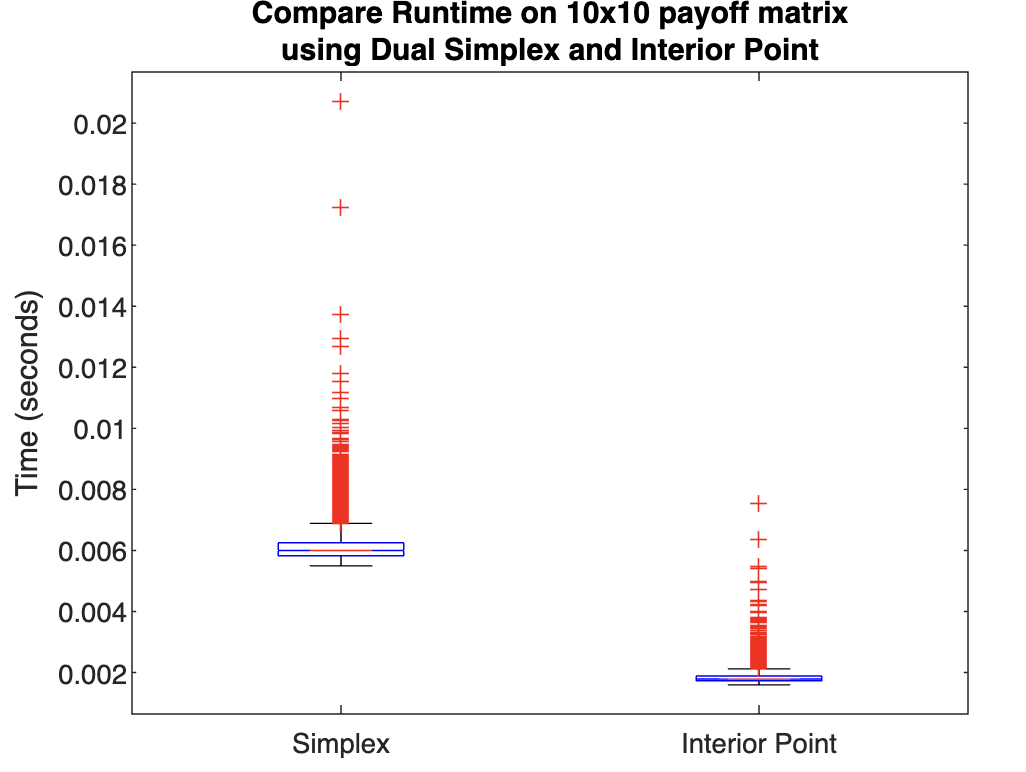
\includegraphics[width=0.45\textwidth]{images/10x10.png}
    \caption{Compare Runtime on 10x10 utility matrix using Dual and Interior Point Method}
    \label{fig:10x10}
\end{figure}
\begin{figure}[!htb]
    \centering
    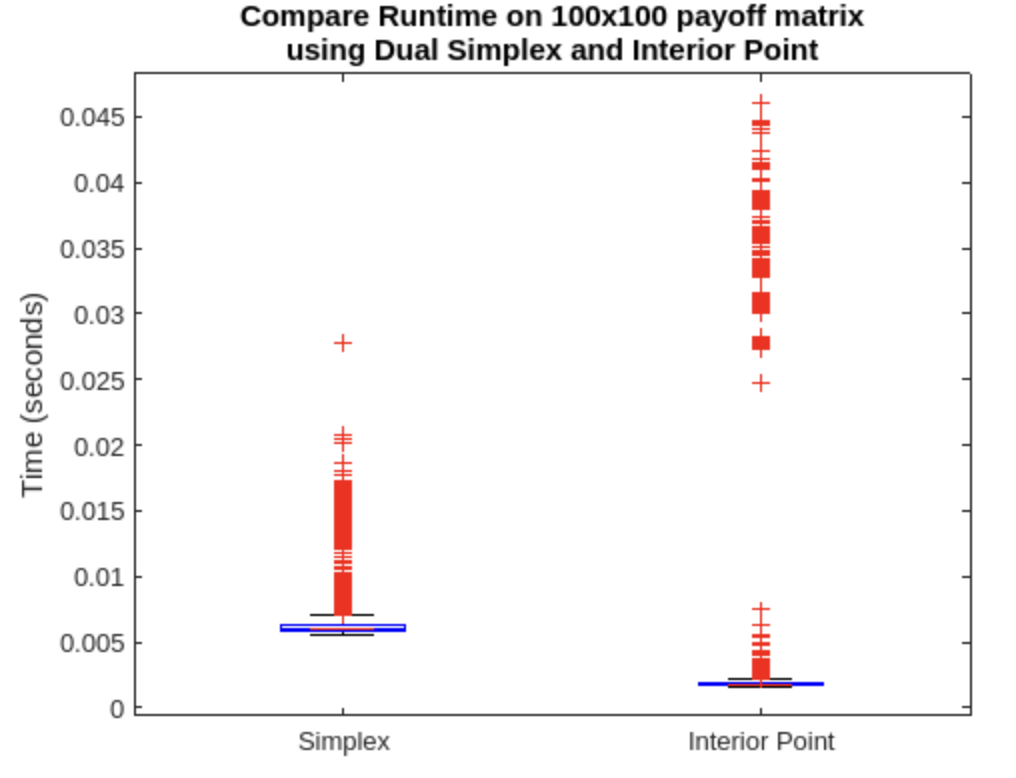
\includegraphics[width=0.45\textwidth]{images/100x100.png}
    \caption{Compare Runtime on 100x100 utility matrix using Dual and Interior Point Method}
    \label{fig:100x100}
\end{figure}

\section{Discussion}
A natural extension of Zero-sum Game is to General-sum Game, where, depending on the actions of players, the total utility of the two players might change. John Nash proves that in such a game, there always exist at least one Nash Equilibrium. 
\begin{theorem}[Nash's Theorem]
    In any game involving a finite number of players, where each player have \textit{mixed strategy} from a finite set of pure strategies, there exists at least one Nash equilibrium.
\end{theorem}
Nash's Theorem, however, is only existential, that is, it does not points out the in ways in which we can construct a mixed-strategy Nash Equilibrium in General-sum Game. Current approach includes formulating the game as a \textit{linear complementarity problem}, then uses graph-search algorithm to seek for \textit{best response strategies}, which form the \textit{support} for the mixed-strategy. However, at the moment, even the state-of-the-art algorithm for this purpose - the Lemke-Howson, is not polynomial in worst case.
\section*{acknowledgement}
    We would like to thank Prof. Hieu Nguyen at Fulbright University Vietnam for providing us with a primer on linear programming and duality in MATH310: Optimization.

\bibliographystyle{IEEEtran}
\bibliography{IEEEabrv,opti_citation}

\end{document}